\section{Схема вычислительного эксперимента}

Эксперимент с программой на нашем компьютере.

\begin{figure}[H]
    \centering
    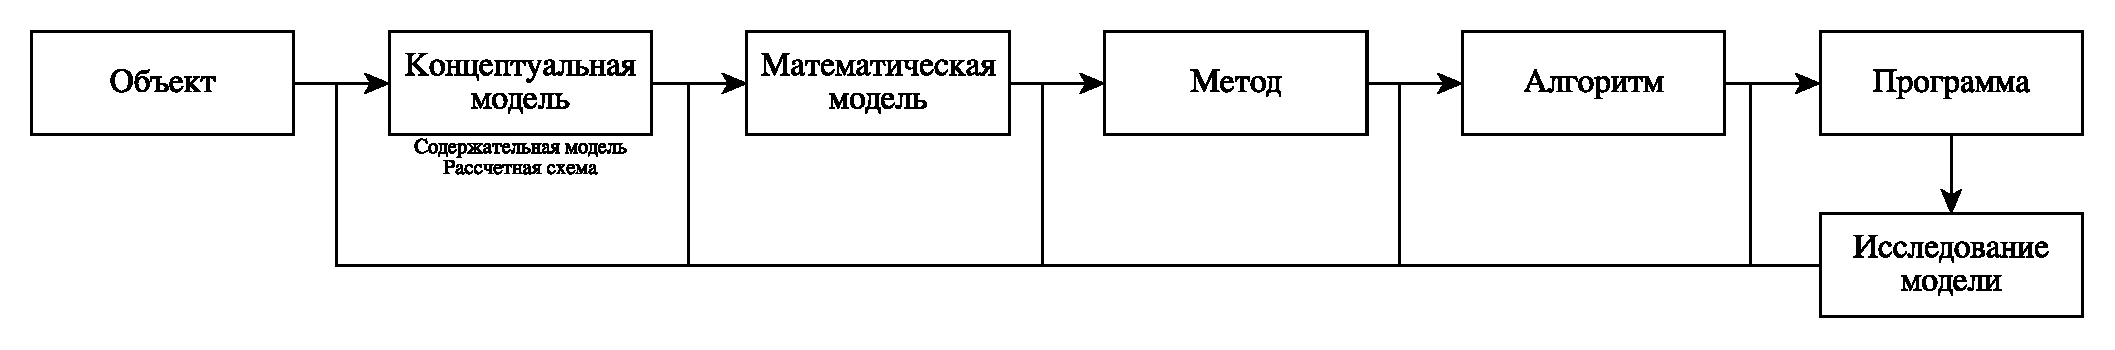
\includegraphics[scale=0.5]{img/schema.pdf}
\end{figure}

\section{Методы получения модели}

\begin{enumerate}
    \item На основе фундаментальных законов природы (сымый хороший)
    \item На основе вариационных принципов
    \item Построение иерархии моделей (снизу вверх и сверху вниз)
    \item Метод аналогий
\end{enumerate}

\section{Источники погрешности при вычислении}

\begin{enumerate}
    \item Погрешность модели
    \item Погрешность исходных данных (неустранимая)
    \item Погрешность метода
\end{enumerate}

\section{Понятие о корректности постановке задачи}

Задача называется \textbf{корректно поставленной}, если ее
решение существует единственно и устойчиво по входным данным.
Устойчивость по входных данным  означает, что малое изменение
входных данных приводит к малому изменению результата.
Если это не так, то тогда задача неустойчива.

Задача, в которых формально устойчивы, то есть при большом $C$
с небольшими изменениями $\delta x$ большие изменения результата.
$\delta y = C \delta x$
